\qquad Conforme orientado no enunciado do trabalho, a análise do Shell
Sort não segue o mesmo roteiro de contagem de instruções aplicado aos
demais algoritmos, pois sua complexidade depende diretamente da
sequência de intervalos (\textit{gaps}) utilizada. Em vez disso, foi
realizada uma pesquisa bibliográfica sobre a complexidade da sequência
de gaps efetivamente utilizada na implementação (a sequência original
de Shell: tamanho/2, tamanho/4, ..., 1), cujo conteúdo manuscrito deve
ser inserido a seguir, substituindo a imagem de exemplo abaixo.

\begin{figure}[htbp]
    \centering
    % Substitua o arquivo abaixo pela digitalizacao da pesquisa/analise manuscrita
    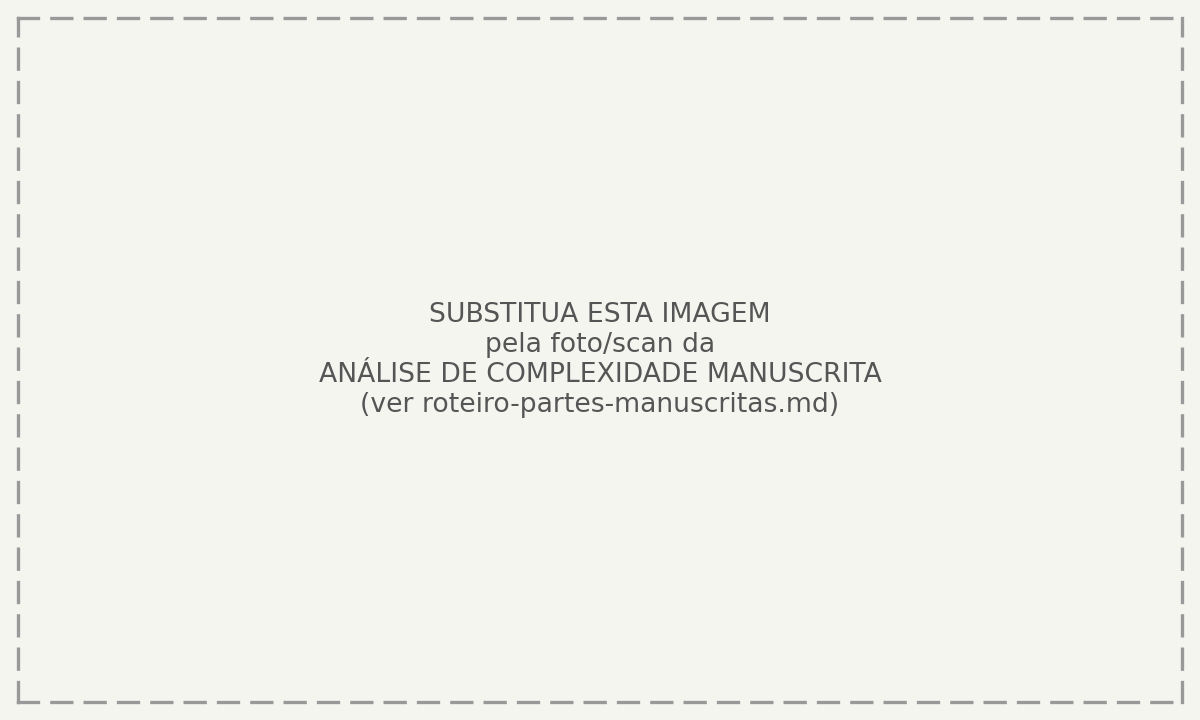
\includegraphics[width=14cm]{Imagens/Shell Sort/analise_complexidade.png}
    \caption{Pesquisa e análise de complexidade manuscrita do algoritmo Shell Sort}
    \label{fig:analise_complexidade_shell}
\end{figure}

\qquad Em resumo, a sequência de Shell utilizada tem pior caso teórico
$\Theta(n^2)$ (resultado devido a Donald Knuth), mas esse pior caso
exige uma disposição de dados especificamente construída para isso —
uma simples entrada decrescente não é suficiente para atingi-lo, pois
qualquer subsequência de um vetor decrescente também está em ordem
decrescente, o que mantém os deslocamentos de cada passada limitados.
Por isso, tanto a entrada crescente quanto a decrescente apresentaram,
nos testes deste trabalho, comportamento próximo de $O(n \log n)$,
enquanto a entrada randômica apresentou um comportamento empírico
intermediário, sem uma fórmula fechada simples de caso médio conhecida
na literatura para esta sequência específica de gaps. Ainda assim,
mesmo utilizando a sequência mais simples possível, o Shell Sort
superou folgadamente os demais algoritmos deste trabalho em todos os
tipos de entrada testados, como mostram os resultados da próxima
seção.
